\protect\hyperlink{main-nav}{≡} \protect\hyperlink{close-nav}{×}

\hypertarget{section-4.2-calculus-of-functions-of-two-variables}{%
\section{Section 4.2: Calculus of Functions of Two
Variables}\label{section-4.2-calculus-of-functions-of-two-variables}}

Now that you have some familiarity with functions of two variables, it's
time to start applying calculus to help us solve problems with them. In
Chapter 2, we learned about the derivative for functions of two
variables. Derivatives told us about the shape of the function, and let
us find local max and min -- we want to be able to do the same thing
with a function of two variables.

First let's think. Imagine a surface, the graph of a function of two
variables. Imagine that the surface is smooth and has some hills and
some valleys. Concentrate on one point on your surface. What do we want
the derivative to tell us? It ought to tell us how quickly the height of
the surface changes as we move\ldots{} Wait, which direction do we want
to move? This is the reason that derivatives are more complicated for
functions of several variables -- there are so many (in fact, infinitely
many) directions we could move from any point.

It turns out that our idea of fixing one variable and watching what
happens to the function as the other changes is the key to extending the
idea of derivatives to more than one variable.

\hypertarget{partial-derivatives}{%
\subsection{Partial Derivatives}\label{partial-derivatives}}

To view this video please enable JavaScript, and consider upgrading to a
web browser that \href{http://videojs.com/html5-video-support/}{supports
HTML5 video}

\hypertarget{partial-derivatives-1}{%
\paragraph{Partial Derivatives}\label{partial-derivatives-1}}

Suppose that \textbackslash{}(z = f(x, y)\textbackslash{}) is a function
of two variables.

The \textbf{partial derivative of \textbackslash{}(f\textbackslash{})
with respect to \textbackslash{}(x\textbackslash{})} is the derivative
of the function \textbackslash{}(f(x,y)\textbackslash{}) where we think
of \textbackslash{}(x\textbackslash{}) as the only variable and act as
if \textbackslash{}(y\textbackslash{}) is a constant.

The \textbf{partial derivative of \textbackslash{}(f\textbackslash{})
with respect to \textbackslash{}(y\textbackslash{})} is the derivative
of the function \textbackslash{}(f(x,y)\textbackslash{}) where we think
of \textbackslash{}(y\textbackslash{}) as the only variable and act as
if \textbackslash{}(x\textbackslash{}) is a constant.

The ``with respect to \textbackslash{}(x\textbackslash{})'' or ``with
respect to \textbackslash{}(y\textbackslash{})'' part is really
important -- you have to know and tell which variable you are thinking
of as \emph{THE} variable.

\hypertarget{geometrically}{%
\subparagraph{Geometrically}\label{geometrically}}

Geometrically the partial derivative with respect to
\textbackslash{}(x\textbackslash{}) gives the slope of the curve as you
travel along a cross-section, a curve on the surface parallel to the
\textbackslash{}(x\textbackslash{})-axis. The partial derivative with
respect to \textbackslash{}(y\textbackslash{}) gives the slope of the
cross-section parallel to the \textbackslash{}(y\textbackslash{})-axis.

\hypertarget{notation-for-the-partial-derivative}{%
\subparagraph{Notation for the Partial
Derivative}\label{notation-for-the-partial-derivative}}

The partial derivative of \textbackslash{}(z = f(x,y)\textbackslash{})
with respect to \textbackslash{}(x\textbackslash{}) is written as
\textbackslash{}{[} f\_x(x,y) \textbackslash{}{]} or simply
\textbackslash{}{[} f\_x
\textbackslash{}quad\textbackslash{}text\{or\}\textbackslash{}quad z\_x.
\textbackslash{}{]}

The Leibniz notation is \textbackslash{}{[}
\textbackslash{}frac\{\textbackslash{}partial
f\}\{\textbackslash{}partial x\} \textbackslash{}{]} or
\textbackslash{}{[} \textbackslash{}frac\{\textbackslash{}partial
z\}\{\textbackslash{}partial x\}. \textbackslash{}{]}

We use an adaptation of the \textbackslash{}(
\textbackslash{}frac\{\textbackslash{}partial
z\}\{\textbackslash{}partial x\} \textbackslash{}) notation to mean
``find the partial derivative of
\textbackslash{}(f(x,y)\textbackslash{}) with respect to
\textbackslash{}(x\textbackslash{})'': \textbackslash{}{[}
\textbackslash{}frac\{\textbackslash{}partial\}\{\textbackslash{}partial
x\}\textbackslash{}left(f(x,y)\textbackslash{}right)=\textbackslash{}frac\{\textbackslash{}partial
f\}\{\textbackslash{}partial x\} \textbackslash{}{]}

\hypertarget{to-estimate-a-partial-derivative-from-a-table-or-contour-diagram}{%
\subparagraph{To estimate a partial derivative from a table or contour
diagram}\label{to-estimate-a-partial-derivative-from-a-table-or-contour-diagram}}

The partial derivative with respect to
\textbackslash{}(x\textbackslash{}) can be approximated by looking at an
average rate of change, or the slope of a secant line, over a very tiny
interval in the \textbackslash{}(x\textbackslash{})-direction (holding
\textbackslash{}(y\textbackslash{}) constant). The tinier the interval,
the closer this is to the true partial derivative.

\hypertarget{to-compute-a-partial-derivative-from-a-formula}{%
\subparagraph{To compute a partial derivative from a
formula}\label{to-compute-a-partial-derivative-from-a-formula}}

If \textbackslash{}(f(x,y)\textbackslash{}) is given as a formula, you
can find the partial derivative with respect to
\textbackslash{}(x\textbackslash{}) algebraically by taking the ordinary
derivative thinking of \textbackslash{}(x\textbackslash{}) as the only
variable (holding \textbackslash{}(y\textbackslash{}) fixed).

Of course, \textbf{everything here works the same way if we're trying to
find the partial derivative with respect to
\textbackslash{}(y\textbackslash{})} -- just think of
\textbackslash{}(y\textbackslash{}) as your only variable and act as if
\textbackslash{}(x\textbackslash{}) is constant.

The idea of a partial derivative works perfectly well for a function of
several variables: you focus on one variable to be \emph{THE} variable
and act as if all the other variables are constants.

To view this video please enable JavaScript, and consider upgrading to a
web browser that \href{http://videojs.com/html5-video-support/}{supports
HTML5 video}

\hypertarget{example-1}{%
\paragraph{Example 1}\label{example-1}}

Here is a contour diagram for a function
\textbackslash{}(g(x,y)\textbackslash{}).

\begin{figure}
\centering
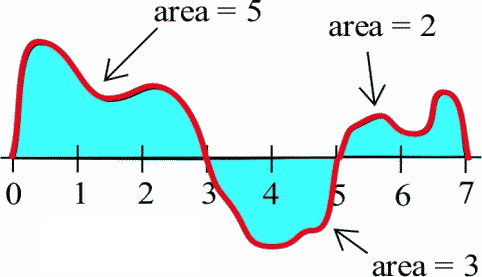
\includegraphics{images/image026.png}
\caption{}
\end{figure}

Use the diagram to answer the following questions:

\begin{enumerate}
\tightlist
\item
  Estimate \textbackslash{}( g\_x(3,5) \textbackslash{}) and
  \textbackslash{}( g\_y(3,5) \textbackslash{}).
\item
  Where on this diagram is \textbackslash{}( g\_x \textbackslash{})
  greatest? Where is \textbackslash{}( g\_y \textbackslash{}) greatest?
\end{enumerate}

\begin{enumerate}
\item
  \textbackslash{}( g\_x(3,5) \textbackslash{}) means we're thinking of
  \textbackslash{}(x\textbackslash{}) as the only variable, so we'll
  hold \textbackslash{}(y\textbackslash{}) fixed at \textbackslash{}(y =
  5\textbackslash{}). That means we'll be looking along the horizontal
  line \textbackslash{}(y = 5\textbackslash{}). To estimate
  \textbackslash{}(g\_x\textbackslash{}), we need two function values.
  (3, 5) lies on the contour line, so we know that \textbackslash{}(g(3,
  5) = 0.6\textbackslash{}). The next point as we move to the right is
  \textbackslash{}(g(4.2,5) = 0.7\textbackslash{}).

  Now we can find the average rate of change: \textbackslash{}{[}
  \textbackslash{}begin\{align*\} \textbackslash{}text\{Average rate of
  change \}=\& \textbackslash{}frac\{\textbackslash{}text\{(change in
  output)\}\}\{\textbackslash{}text\{(change in input)\}\}
  \textbackslash{}\textbackslash{} =\&
  \textbackslash{}frac\{\textbackslash{}Delta g\}\{\textbackslash{}Delta
  x\}\textbackslash{}\textbackslash{} =\&
  \textbackslash{}frac\{0.7-0.6\}\{4.2-3\}\textbackslash{}\textbackslash{}
  =\& \textbackslash{}frac\{1\}\{12\}\textbackslash{}approx 0.083
  \textbackslash{}end\{align*\} \textbackslash{}{]} We can do the same
  thing by going to the next point we can read to the left, which is
  \textbackslash{}(g(2.4,5) = 0.5\textbackslash{}). Then the average
  rate of change is \textbackslash{}{[}
  \textbackslash{}frac\{\textbackslash{}Delta g\}\{\textbackslash{}Delta
  x\}=\textbackslash{}frac\{0.5-0.6\}\{2.4-3\}=\textbackslash{}frac\{1\}\{6\}\textbackslash{}approx
  0.167.\textbackslash{}{]}

  Either of these would be a fine estimate of \textbackslash{}(
  g\_x(3,5) \textbackslash{}) given the information we have, or we could
  take their average. We can estimate that \textbackslash{}(
  g\_x(3,5)\textbackslash{}approx 0.125 \textbackslash{}).

  Estimate \textbackslash{}( g\_y(3,5) \textbackslash{}) the same way,
  but moving on the vertical line. Using the next point up, we get the
  average rate of change is \textbackslash{}{[}
  \textbackslash{}frac\{\textbackslash{}Delta g\}\{\textbackslash{}Delta
  y\}=\textbackslash{}frac\{0.7-0.6\}\{5.8-5\}=\textbackslash{}frac\{1\}\{8\}=0.125.\textbackslash{}{]}
  Using the next point down, we get \textbackslash{}{[}
  \textbackslash{}frac\{\textbackslash{}Delta g\}\{\textbackslash{}Delta
  y\}=\textbackslash{}frac\{0.5-0.6\}\{4.5-5\}=\textbackslash{}frac\{1\}\{5\}=0.2.\textbackslash{}{]}
  Taking their average, we estimate \textbackslash{}(
  g\_y(3,5)\textbackslash{}approx 0.1625 \textbackslash{}).
\item
  \textbackslash{}( g\_x \textbackslash{}) means
  \textbackslash{}(x\textbackslash{}) is our only variable, and we're
  thinking of \textbackslash{}(y\textbackslash{}) as a constant. So
  we're thinking about moving across the diagram on horizontal lines.
  \textbackslash{}( g\_x \textbackslash{}) will be greatest when the
  contour lines are closest together, i.e., when the surface is steepest
  -- then the denominator in \textbackslash{}(
  \textbackslash{}frac\{\textbackslash{}Delta g\}\{\textbackslash{}Delta
  x\} \textbackslash{}) will be small, so \textbackslash{}(
  \textbackslash{}frac\{\textbackslash{}Delta g\}\{\textbackslash{}Delta
  x\} \textbackslash{}) will be big. Scanning the graph, we can see that
  the contour lines are closest together when we head to the left or to
  the right from about (0.5, 8) and (9, 8). So \textbackslash{}( g\_x
  \textbackslash{}) is greatest at about (0.5, 8) and (9, 8). For
  \textbackslash{}( g\_y \textbackslash{}), we want to look at vertical
  lines. \textbackslash{}( g\_y \textbackslash{}) is greatest at about
  (5, 3.8) and (5, 12).
\end{enumerate}

To view this video please enable JavaScript, and consider upgrading to a
web browser that \href{http://videojs.com/html5-video-support/}{supports
HTML5 video}

\hypertarget{example-2}{%
\paragraph{Example 2}\label{example-2}}

Cold temperatures feel colder when the wind is blowing. Windchill is the
perceived temperature, and it depends on both the actual temperature and
the wind speed -- a function of two variables! You can read more about
windchill at \url{http://www.nws.noaa.gov/om/windchill/}. Below is a
table that shows the perceived temperature for various temperatures and
windspeeds.

\begin{figure}
\centering
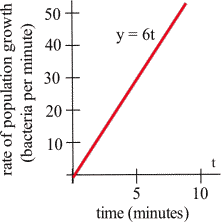
\includegraphics{images/image045.png}
\caption{(Table courtesy of the National Weather Service,
\url{http://www.nws.noaa.gov/om/windchill/images/windchill.gif}.)}
\end{figure}

Note that they also include the formula, but for this example we'll use
the information in the table.

\begin{enumerate}
\tightlist
\item
  What is the perceived temperature when the actual temperature is 25°F
  and the wind is blowing at 15 miles per hour?
\item
  Suppose the actual temperature is 25°F. Use information from the table
  to describe how the perceived temperature would change if the wind
  speed increased from 15 miles per hour?
\end{enumerate}

\begin{enumerate}
\item
  Reading the table, we see that the perceived temperature is 13°F
\item
  This is a question about a partial derivative. We're holding the
  temperature (\textbackslash{}(T\textbackslash{})) fixed at 25°F, and
  asking what happens as wind speed
  (\textbackslash{}(V\textbackslash{})) increases from 15 miles per
  hour. We're thinking of \textbackslash{}(V\textbackslash{}) as the
  only variable, so we want
  \textbackslash{}(\textbackslash{}text\{WindChillV\} =
  W\_V\textbackslash{}) when \textbackslash{}(T = 25\textbackslash{})
  and \textbackslash{}(V = 15\textbackslash{}). We'll find the average
  rate of change by looking in the column where \textbackslash{}(T =
  25\textbackslash{}) and letting \textbackslash{}(V\textbackslash{})
  increase, and use that to approximate the partial derivative.
  \textbackslash{}{[} W\_V\textbackslash{}approx
  \textbackslash{}frac\{\textbackslash{}Delta W\}\{\textbackslash{}Delta
  V\}=\textbackslash{}frac\{11-13\}\{20-15\}=-0.4 \textbackslash{}{]}

  What are the units? \textbackslash{}(W\textbackslash{}) is measured in
  °F and \textbackslash{}(V\textbackslash{}) is measured in mph, so the
  units here are °F/mph. And that lets us describe what happens: The
  perceived temperature would decrease by about 0.4°F for each mph
  increase in wind speed.
\end{enumerate}

\hypertarget{example-3}{%
\paragraph{Example 3}\label{example-3}}

Find \textbackslash{}( f\_x \textbackslash{}) and \textbackslash{}( f\_y
\textbackslash{}) at the points (0, 0) and (1, 1) if \textbackslash{}(
f(x,y)=x\^{}2-4xy+4y\^{}2 \textbackslash{}).

To find \textbackslash{}( f\_x \textbackslash{}), take the ordinary
derivative of \textbackslash{}(f\textbackslash{}) with respect to
\textbackslash{}(x\textbackslash{}), acting as if
\textbackslash{}(y\textbackslash{}) is constant: \textbackslash{}{[}
f\_x(x,y)=2x-4y. \textbackslash{}{]}

Note that the derivative of the \textbackslash{}( 4y\^{}2
\textbackslash{}) term with respect to
\textbackslash{}(x\textbackslash{}) is zero because it's a constant (as
far as \textbackslash{}( x \textbackslash{}) is concerned).

Similarly, \textbackslash{}{[} f\_y(x,y)=-4x+8y. \textbackslash{}{]}

Now we can evaluate these at the points:

\textbackslash{}( f\_x(0,0)=0 \textbackslash{}) and \textbackslash{}(
f\_y(0,0)=0 \textbackslash{}); this tells us that the cross sections
parallel to the \textbackslash{}(x\textbackslash{})- and
\textbackslash{}(y\textbackslash{})- axes are both flat at (0,0).

\textbackslash{}( f\_x(1,1)=-2 \textbackslash{}) and \textbackslash{}(
f\_y(1,1)=4 \textbackslash{}); this tells us that above the point (1,
1), the surface decreases if we move to more positive
\textbackslash{}(x\textbackslash{}) values and increases if we move to
more positive \textbackslash{}(y\textbackslash{}) values.

\hypertarget{example-4}{%
\paragraph{Example 4}\label{example-4}}

Find \textbackslash{}( \textbackslash{}frac\{\textbackslash{}partial
f\}\{\textbackslash{}partial x\} \textbackslash{}) and \textbackslash{}(
\textbackslash{}frac\{\textbackslash{}partial
f\}\{\textbackslash{}partial y\} \textbackslash{}) if \textbackslash{}(
f(x,y)=\textbackslash{}frac\{e\^{}\{x+y\}\}\{y\^{}3+y\}+y\textbackslash{}ln(y)
\textbackslash{}).

\textbackslash{}( \textbackslash{}frac\{\textbackslash{}partial
f\}\{\textbackslash{}partial x\} \textbackslash{}) means
\textbackslash{}(x\textbackslash{}) is our only variable, we're thinking
of \textbackslash{}(y\textbackslash{}) as a constant. Then we'll just
find the ordinary derivative. From \textbackslash{}(x\textbackslash{})'s
point of view, this is an exponential function, divided by a constant,
with a constant added. The constant pulls out in front, the derivative
of the exponential function is the same thing, and we need to use the
chain rule, so we multiply by the derivative of that exponent (which is
just 1): \textbackslash{}{[}
\textbackslash{}frac\{\textbackslash{}partial
f\}\{\textbackslash{}partial
x\}=\textbackslash{}frac\{1\}\{y\^{}3+y\}e\^{}\{x+y\}.
\textbackslash{}{]}

\textbackslash{}(\textbackslash{}frac\{\textbackslash{}partial
f\}\{\textbackslash{}partial y\}\textbackslash{}) means that we're
thinking of \textbackslash{}(y\textbackslash{}) as the variable, acting
as if \textbackslash{}(x\textbackslash{}) is constant. From
\textbackslash{}(y\textbackslash{})'s point of view,
\textbackslash{}(f\textbackslash{}) is a quotient plus a product, so
we'll need the quotient rule and the product rule: \textbackslash{}{[}
\textbackslash{}begin\{align*\}
\textbackslash{}frac\{\textbackslash{}partial
f\}\{\textbackslash{}partial y\}=\&
\textbackslash{}frac\{(\textbackslash{} )(\textbackslash{}
)-(\textbackslash{} )(\textbackslash{} )\}\{(\textbackslash{}
)\^{}2\}+(\textbackslash{} )(\textbackslash{} )+(\textbackslash{}
)(\textbackslash{} ) \textbackslash{}\textbackslash{} =\&
\textbackslash{}frac\{\textbackslash{}left( e\^{}\{x+y\}(1)
\textbackslash{}right)\textbackslash{}left( y\^{}3+y
\textbackslash{}right)-\textbackslash{}left( e\^{}\{x+y\}
\textbackslash{}right)\textbackslash{}left( 3y\^{}2+1
\textbackslash{}right)\}\{\textbackslash{}left( y\^{}3+y
\textbackslash{}right)\^{}2\}+\textbackslash{}left( 1
\textbackslash{}right)\textbackslash{}left( \textbackslash{}ln(y)
\textbackslash{}right)+\textbackslash{}left( y
\textbackslash{}right)\textbackslash{}left(
\textbackslash{}frac\{1\}\{y\} \textbackslash{}right)
\textbackslash{}end\{align*\} \textbackslash{}{]}

\hypertarget{example-5}{%
\paragraph{Example 5}\label{example-5}}

Find \textbackslash{}( f\_z \textbackslash{}) if \textbackslash{}(
f(x,y,z,w)=35x\^{}2w-\textbackslash{}frac\{1\}\{z\}+yz\^{}2
\textbackslash{}).

\textbackslash{}( f\_z \textbackslash{}) means we act as if
\textbackslash{}(z\textbackslash{}) is our only variable, so we'll act
as if all the other variables (\textbackslash{}(x\textbackslash{}),
\textbackslash{}(y\textbackslash{}), and
\textbackslash{}(w\textbackslash{})) are constants and take the ordinary
derivative: \textbackslash{}{[}
f\_z(x,y,z,w)=\textbackslash{}frac\{1\}\{z\^{}2\}+2yz.
\textbackslash{}{]}

To view this video please enable JavaScript, and consider upgrading to a
web browser that \href{http://videojs.com/html5-video-support/}{supports
HTML5 video}

\hypertarget{using-partial-derivatives-to-estimate-function-values}{%
\subsection{Using Partial Derivatives to Estimate Function
Values}\label{using-partial-derivatives-to-estimate-function-values}}

We can use the partial derivatives to estimate values of a function. The
geometry is similar to the tangent line approximation in one variable.
Recall the one-variable case: if \textbackslash{}(x\textbackslash{}) is
close enough to a known point \textbackslash{}(a\textbackslash{}), then
\textbackslash{}{[} f(x)\textbackslash{}approx f(a)+f'(a)(x-a).
\textbackslash{}{]} In two variables, we do the same thing in both
directions at once:

\hypertarget{approximating-function-values-with-partial-derivatives}{%
\paragraph{Approximating Function Values with Partial
Derivatives}\label{approximating-function-values-with-partial-derivatives}}

To approximate the value of \textbackslash{}(f(x, y)\textbackslash{}),
find some point \textbackslash{}((a, b)\textbackslash{}) where

\begin{enumerate}
\tightlist
\item
  \textbackslash{}((x, y)\textbackslash{}) and \textbackslash{}((a,
  b)\textbackslash{}) are close, that is,
  \textbackslash{}(x\textbackslash{}) and
  \textbackslash{}(a\textbackslash{}) are close and
  \textbackslash{}(y\textbackslash{}) and
  \textbackslash{}(b\textbackslash{}) are close.
\item
  You know the exact values of \textbackslash{}(f(a, b)\textbackslash{})
  and both partial derivatives there.
\end{enumerate}

Then \textbackslash{}{[} f(x,y)\textbackslash{}approx
f(a,b)+f\_x(a,b)(x-a)+f\_y(a,b)(y-b). \textbackslash{}{]}

Notice that the total change in \textbackslash{}(f\textbackslash{}) is
being approximated by adding the approximate changes coming from the
\textbackslash{}(x\textbackslash{}) and
\textbackslash{}(y\textbackslash{}) directions. Another way to look at
the same formula: \textbackslash{}{[} \textbackslash{}Delta
f\textbackslash{}approx f\_x\textbackslash{}Delta
x+f\_y\textbackslash{}Delta y. \textbackslash{}{]}

How close is close? It depends on the shape of the graph of
\textbackslash{}(f\textbackslash{}). In general, the closer the better.

\hypertarget{example-6}{%
\paragraph{Example 6}\label{example-6}}

Use partial derivatives to estimate the value of \textbackslash{}(
f(x,y)=x\^{}2-4xy+4y\^{}2 \textbackslash{}) at (0.9, 1.1).

Note that the point (0.9, 1.1) is close to an ``easy'' point, (1, 1). In
fact, we already worked out the partial derivatives at (1, 1):
\textbackslash{}( f\_x(x,y)=2x-4y \textbackslash{}) so \textbackslash{}(
f\_x(1,1)=-2 \textbackslash{}), and \textbackslash{}( f\_y(x,y)=-4x+8y
\textbackslash{}) so \textbackslash{}( f\_y(1,1)=4 \textbackslash{}). We
also know that \textbackslash{}( f(1,1)=1 \textbackslash{}).

So, \textbackslash{}{[} f(0.9,1.1)\textbackslash{}approx
1-2(-0.1)+4(0.1)=1.6. \textbackslash{}{]}

Note that in this example it would have been possible to simply compute
the exact answer: \textbackslash{}{[}
f(0.9,1.1)=(0.9)\^{}2-4(0.9)(1.1)+4(1.1)\^{}2=1.69. \textbackslash{}{]}
Our estimate is not perfect, but it's pretty close.

To view this video please enable JavaScript, and consider upgrading to a
web browser that \href{http://videojs.com/html5-video-support/}{supports
HTML5 video}

\hypertarget{example-7}{%
\paragraph{Example 7}\label{example-7}}

Here is a contour diagram for a function
\textbackslash{}(g(x,y)\textbackslash{}). Use partial derivatives to
estimate the value of \textbackslash{}(g(3.2, 4.7)\textbackslash{}).

\begin{figure}
\centering
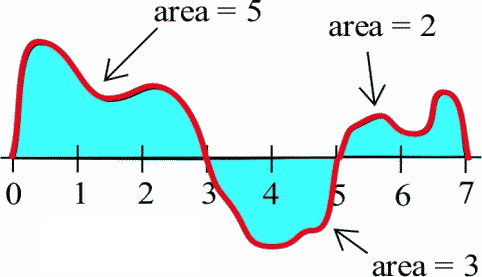
\includegraphics{images/image026.png}
\caption{}
\end{figure}

This is the same diagram from before, so we already estimated the value
of the function and the partial derivatives at the nearby point (3,5).
\textbackslash{}(g(3, 5)\textbackslash{}) is 0.6, our estimate of
\textbackslash{}( g\_x(3,5)\textbackslash{}approx 0.125
\textbackslash{}), and our estimate of \textbackslash{}(
g\_y(3,5)\textbackslash{}approx 0.1625 \textbackslash{}). So
\textbackslash{}{[} g(3.2,4.7)\textbackslash{}approx
0.6+(0.125)(0.2)+(0.1625)(-0.3)=0.57625. \textbackslash{}{]} Note that
in this example we have no way to know how close our estimate is to the
actual value.

\begin{longtable}[]{@{}ll@{}}
\toprule
\endhead
\href{section4-1.php}{← Previous Section} & \href{section4-3.php}{Next
Section →}\tabularnewline
\bottomrule
\end{longtable}
